\section{Closed-loop identification issue with \ac{DeePC}}\label{sec:CL_ID_issue}
% Correlation between inputs and preceding noise produces a bias for the underlying identification task in \ac{DeePC}~\citep{Dinkla2023}. This section demonstrates this issue for adaptive controller implementations using simulations.
%
This section demonstrates that adaptive \ac{DeePC} implementations (unlike \ac{CL-DeePC}) are affected by identification bias that arises from correlation between inputs and preceding noise during closed-loop operation.

\subsection{Motivating example}
To illustrate the resulting potential performance degradation of \ac{DeePC} in an adaptive setting, consider Fig.~\ref{fig:CL_Problem_Solution}. \ac{DeePC} clearly manages considerably worse reference tracking performance w.r.t. \ac{CL-DeePC}, which seems to perform comparably to the oracle. At first, all of the data that the data-driven controllers rely on derives from open-loop operation. Due to the adaptive nature of the controller implementation, after $\bar{N}$ time steps, all of the employed data derives from closed-loop operation. The reference tracking ability of \ac{DeePC} appears to decrease as the amount of employed closed-loop data increases. Thereafter, a cyclical behaviour may be observed for \ac{DeePC}: large reference tracking errors that result from, e.g., the closed-loop identification issue momentarily increase the effective signal to noise ratio and thereby temporarily improve the obtained reference tracking performance again.
% ------------------------- Figure --------------------------
\begin{figure}[b!]
\begin{center}%
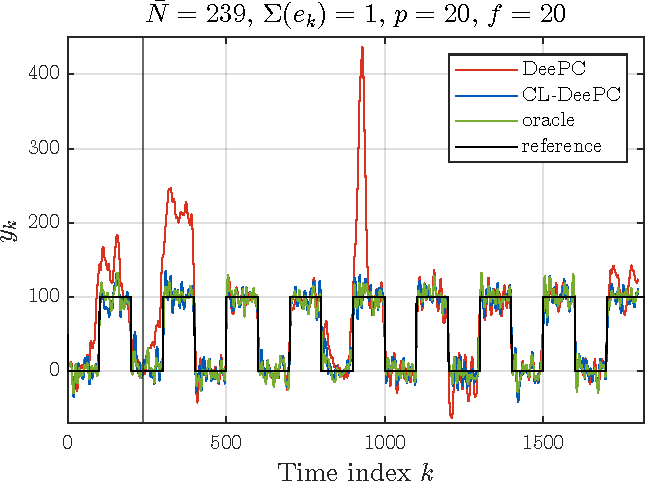
\includegraphics[width=\columnwidth]{results/figures/DeePC_CL_ID_issue_Re_1_Nbar_239_p_20_f_20_Ru_1_Rdu_0_Q_100_R_0_dR_10.pdf}    % The printed column  
\caption{Reference tracking by adaptive \ac{DeePC} and \ac{CL-DeePC} using \ac{IVs}. After the vertical line at $\bar{N}$ all used data originates from operation in closed-loop. \ac{DeePC} displays worse reference tracking performance than \ac{CL-DeePC}, in part due to a closed-loop identification problem.}% width is 8.4 cm.
\label{fig:CL_Problem_Solution}%                                 % Size the figures 
\end{center}%                                 % accordingly.
\end{figure}%
% -----------------------------------------------------------

\subsection{Correlation between inputs and noise}
This section demonstrates the existence of correlation between inputs and preceding noise during closed-loop operation in an adaptive setting by means of simulations. Following the preceding consistency proof in \secref{sec:proof_IVs}, the correlation matrix of interest is given by $\frac{1}{N}E_{i_p,f_\mathrm{ID},N}\begin{bmatrix}U_{i,p,N}^\top & U_{i_p,f_\mathrm{ID},N}^\top\end{bmatrix}$, with $f_\mathrm{ID}=f$ for \ac{DeePC}, and $f_\mathrm{ID}=1$ for \ac{CL-DeePC}. An example of such a correlation matrix, averaged over the closed-loop data obtained from 120 simulations with different noise realizations, is shown by Fig.~\ref{fig:EfUpf_correlation}. Unlike with \ac{CL-DeePC}, the input data used by \ac{DeePC} is correlated with the noise that is inherent to used, preceding output measurements. Although in adaptive data-driven implementations there is a stochastic variability associated with subsequent control policies due to noise, this variability is clearly insufficient to mitigate the closed-loop correlation that arises between inputs and preceding noise in \ac{DeePC}.
% ------------------------- Figure --------------------------
\begin{figure}[b!]
\begin{center}
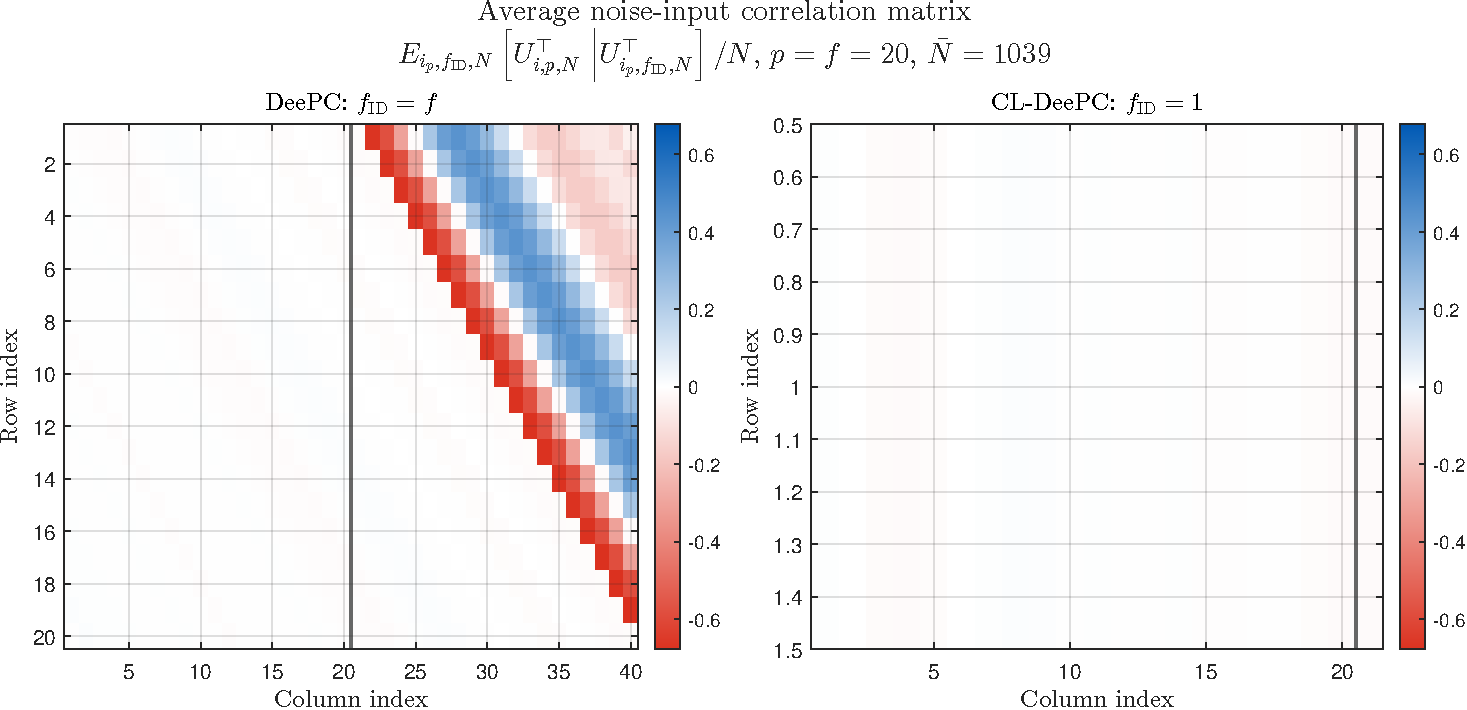
\includegraphics[width=\columnwidth]{results/figures/Correlation_Nbar_1039_p_20_f_20_Re_1_Ru_1_Rdu_0_Q_100_R_0_dR_10.pdf}    % The printed column  
\caption{Noise-input correlation matrix for \ac{DeePC} and \ac{CL-DeePC} averaged over 120 noise realizations. In contrast to \ac{DeePC}, \ac{CL-DeePC} makes use of input data that is uncorrelated with preceding noise.}  % width is 8.4 cm.
\label{fig:EfUpf_correlation}                                 % Size the figures 
\end{center}                                 % accordingly.
\end{figure}
% -----------------------------------------------------------

\subsection{Consistency analysis}
This section demonstrates the consistency (or lack thereof) of the estimators employed by \ac{DeePC} and \ac{CL-DeePC} as a result of closed-loop correlation between inputs and preceding noise. Along the lines of the consistency analysis in \secref{sec:proof_IVs} and~\cite{Dinkla2023} it is to be expected that the implicit matrix estimate of $\mathcal{T}_{f_\mathrm{ID}}^\mathrm{u}$ is inconsistent for \ac{DeePC} ($f_\mathrm{ID}=f$) and consistent for \ac{CL-DeePC} ($f_\mathrm{ID}=1$). Note that for \ac{CL-DeePC}, the estimate of $\mathcal{T}_f^\mathrm{u}$ is implicitly constructed from the sequential construction procedure from \secref{sec:Sequential}. In anticipation of potential amplification of identification errors in the resulting matrix estimate for $\mathcal{T}_f^\mathrm{u}$, to facilitate a fair comparison, the error in $\widehat{\mathcal{T}}_f^\mathrm{u}$ is shown for both data-driven methods by Fig.~\ref{fig:Tuf_consistency}. As expected, as the number of employed past data points $\bar{N}$ increases (together with the number of columns $N=\bar{N}-p-f_\mathrm{ID}+1$), the bias of the \ac{CL-DeePC} estimate keeps decreasing, which indicates that the employed estimate is indeed consistent. In contrast, for \ac{DeePC} the bias does not keep decreasing noticeably beyond around $\bar{N}=400$, indicating that the implicitly employed estimate $\widehat{\mathcal{T}}_f^\mathrm{u}$ is inconsistent.
% ------------------------- Figure --------------------------
\begin{figure}[b!]
\begin{center}
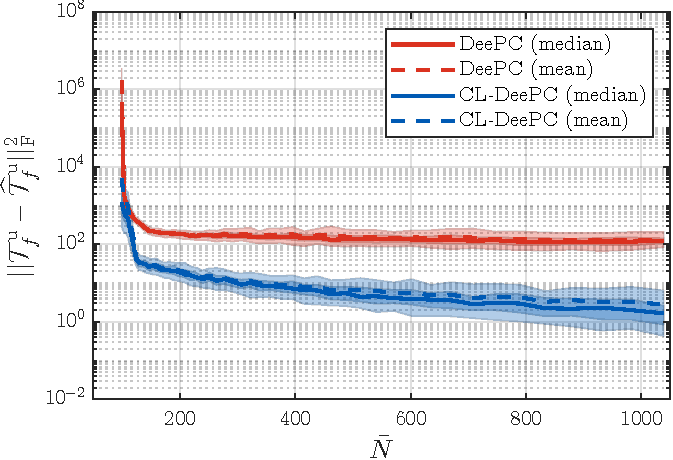
\includegraphics[width=\columnwidth]{results/figures/Consistency_Nbar_99-1039-50_p_20_f_20_Re_1_Ru_1_Rdu_0_Q_100_R_0_dR_10.pdf}    % The printed column  
\caption{Error of the system matrix $\mathcal{T}_f^\mathrm{u}$ (implicitly) estimated by \ac{DeePC} and \ac{CL-DeePC} based exclusively on adaptive closed-loop operation. Increasingly narrow regions around the median contain 80\% and 40\% of the data.}  % width is 8.4 cm.
\label{fig:Tuf_consistency}                                 % Size the figures 
\end{center}                                 % accordingly.
\end{figure}
% -----------------------------------------------------------